\section{Le Deep Q-Learning}

\subsection{Principe du Deep Q-Learning}

Le Q-Learning requiert de stocker les valeurs de la Q-function de quelque manière que ce soit. Notamment, on a utilisé un tableau (la Q-table) dans le jeu des
bâtonnets. Néanmoins, on peut être confronté à des espaces des états de très grande taille : par exemple si les états sont des images (même de taille raisonnable), 
alors on peut imaginer des milliards d'états possibles. Bien que généralement plus restreint, le nombre d'actions est également à l'origine de ce problème puisque la
taille de la matrice est le produit entre le nombre d'états différents et le nombre d'actions possibles. Puisque notre IA jouant à Pong doit recevoir des images du jeu,
il est impensable de stocker chaque valeur en mémoire. Le Deep Q-Learning résout ce problème en remplaçant la Q-table par un réseau neuronal. Son objectif est alors 
d'interpoler la fonction de satisfaction. Cette approximation nous permet d'économiser une importante quantité de mémoire.

On a alors un réseau neuronal qui reçoit en entrée un état et une action pour retourner la satisfaction qui y est associée. Pour pouvoir choisir une action selon
notre algorithme favorisant la plus grande satisfaction, il est nécessaire de connaître la valeur du réseau lorsqu'excité par toutes les actions. Ainsi
le nombre d'évaluations du réseau est égal au nombre d'actions possibles. Cela est d'autant plus inefficace qu'il sera nécessaire d'exécuter cette opération très
régulièrement. Pour régler ce problème, notre réseau ne reçoit plus que l'état en question en entrée. En sortie, le réseau nous donne les satisfactions associées à chaque 
action, de sorte qu'une seule évaluation du réseau suffise à choisir l'action à effectuer.

\begin{figure}[h]
 \centering
 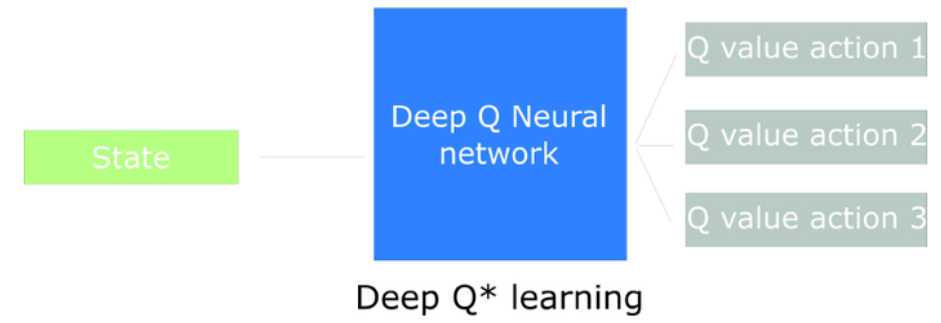
\includegraphics[width=0.7\textwidth]{img/schema_DQL.png}
 \caption{Schéma du Deep Q-Network}
\end{figure}


Lorsque nous réalisons l'apprentissage, nous sélectionnons une transition qui contient l'action choisie à l'instant de la transition. Puisque notre réseau renvoie
toutes les satisfactions, il est important de veiller à ce que le réseau ne réalise la rétropropagation que sur l'action de la transition. Cela peut être 
effectué en remplaçant la valeur voulue pour les autres actions par la valeur calculée, de sorte que l'erreur soit nulle, sauf pour l'action de la transition.
Pour cette dernière, on conserve l'équation \ref{eq:bellman} pour l'expression voulue de la fonction de satisfaction.

Pour faciliter la réalisation de notre algorithme et nous débarrasser des grosses difficultés posées par le réseau neuronal telles que la rétropropagation, il 
a été convenu d'utiliser TensorFlow. Cette bibliothèque Python simplifie considérablement la conception d'un tel algorithme. Néanmoins, pour ne pas trop occulter 
ce qu'il se passe dans le réseau, nous voulons rester suffisamment bas niveau. Ainsi, nous nous interdisons toute surcouche de TensorFlow telle que Keras.


\subsection{Jeu des bâtonnets}

Pour valider notre implémentation du Deep Q-Learning, on le teste sur un jeu simple que l'on sait résoudre : le jeu des bâtonnets. Les règles du jeu sont les mêmes 
que précédemment. Pour la rétropropagation, nous utilisons l'optimiseur Adam particulièrement efficace, avec le taux d'apprentissage 0.001. Le facteur d'actualisation
est conservé, de même que les taux d'exploration. On stocke un maximum de 10000 transitions. Après chaque partie jouée, on apprend sur \emph{toutes} les transitions
enregistrées jusqu'à lors (par minibatch de 32 transitions). Le réseau utilisé possède 4 neurones d'entrée (chaque état est codé binairement), 10 neurones de couche cachée
puis 3 neurones de sortie pour les 3 différentes actions fournies par le jeu. Ce réseau sert à la fois à apprendre sur les transitions et à générer la cible, 
conformément à l'équation \ref{eq:bellman}. Bien que cela ne soit pas l'implémentation la plus optimale, elle suffit pour un jeu aussi simple que celui des bâtonnets.

Notre réseau apprend sur 2000 parties (contre une IA qui est également en train d'apprendre). Pour nous persuader de l'efficacité de notre algorithme, nous reconstituons
la Q-table à l'issue de l'apprentissage en interrogeant le réseau sur les différents états accessibles lors d'une partie. Le résultat est le suivant :

\begin{figure}[h]
\centering
\begin{tabular}{|c|c|c|c|}
\hline
Bâtonnets restants & Prendre 1 bâtonnet & Prendre 2 bâtonnets & Prendre 3 bâtonnets\\
\hline
1 & -0.9966581 & -0.98666275 & -0.99692893\\
\hline
2 & \cellcolor{green} 1.0102367 & -0.9285556 & -0.9973395\\
\hline
3 & 0.1279521 & \cellcolor{green} 1.0385635 & -1.001752\\
\hline
4 & -0.17204374 & -0.1530217 & \cellcolor{green} 1.0058613\\
\hline
5 & -0.509134 & -0.48264277 & -0.49259257\\
\hline
6 & \cellcolor{green} 0.9031452 & -0.11602497 & -0.24787879\\
\hline
7 & 0.10454643 & \cellcolor{green} 0.92308414 & -0.1744315\\
\hline
8 & 0.12821698 & 0.2924267 & \cellcolor{green} 0.9102776\\
\hline
9 & -0.06348622 & -0.0588069 & -0.05864894\\
\hline
10 & \cellcolor{green} 0.82183206 & 0.18388963 & 0.5014814\\
\hline
11 & 0.3764193 & \cellcolor{green} 0.82838273 & 0.14708841\\
\hline
12 & 0.26232004 & 0.44059992 & \cellcolor{green} 0.8352009\\
\hline
\end{tabular}
\caption{Fonction de satisfaction $Q$ approximée par le réseau neuronal}
\label{tab:Qfunction}
\end{figure}

Le tableau \ref{tab:Qfunction} nous prouve que le réseau neuronal a compris la stratégie et l'applique. En effet, pour chaque état, la satisfaction maximale est donnée
au coup prédit par la stratégie. Certaines lignes n'ont pas de maximum évident, car cela correspond à des états où la stratégie nous donne perdant, ainsi les différents
coups se valent. On remarque que la satisfaction dépasse parfois en valeur absolue la récompense effectivement perçue par l'IA, cela peut paraître absurde puisque cette 
récompense est l'objectif final, mais peut s'expliquer par le fait que le réseau ne fait qu'une approximation, et ne calcule donc pas la Q-function exactement.
Néanmoins l'erreur reste assez faible. Enfin, on remarque que la satisfaction accordée aux bons coups est meilleure lorsque l'on est proche de la fin de la partie.
Cela provient du fait que la propagation de la récompense favorise les états proches de celui où la satisfaction est effectivement attribuée. Quoiqu'il en soit, notre IA
respecte parfaitement la stratégie, qu'elle a pu apprendre en moins de 10 minutes malgré une implémentation imparfaite.


\subsection{Changements effectués pour le passage à Pong}

Maintenant que nous nous sommes assurés de la fiabilité de notre implémentation du Deep Q-Learning sur le jeu des bâtonnets, nous voulons l'appliquer sur Pong.
Pong est bien plus compliqué que le jeu des bâtonnets, ainsi plusieurs modifications seront nécessaires.

\subsubsection{Deux Deep Q-Networks}
\label{section:2networks}

Lorsque nous réalisons la rétropropagation, nous devons connaître l'objectif de notre réseau. Celui-ci est donné par l'équation \ref{eq:bellman}. Ainsi, il est
nécessaire de faire une propagation vers l'avant pour évaluer l'objectif de notre réseau. Notre réseau se ``pourchasse'' donc lui-même. Cela peut mener à de gros 
problèmes de convergence, voire à une instabilité du réseau. Cela n'avait pas été observé précédemment à cause de la simplicité du jeu en question.

L'instabilité du réseau se caractérise par deux choses d'après nos observations. Tout d'abord, le Deep Q-Network ignore totalement l'entrée qui lui est donnée,
il retourne toujours les mêmes satisfactions (précision de $10^{-6}$ pourtant !). De plus, les satisfactions accordées à chaque action diffèrent très peu
(une différence de quelques unités de $10^{-6}$). Ainsi, notre réseau ne sait pas quelle action choisir, l'une est choisie par défaut. Et pourtant, notre réseau
décide de s'y tenir quoiqu'il arrive. Cela se conclut par, ou bien, une immobilité de notre IA, ou bien, une insistance sur l'un des mouvements (c'est-à-dire notre
IA se coince sur l'un des rebords du plateau de jeu et y reste pendant toute la partie).

Pour éviter ce problème, nous considérons deux réseaux différents. Le réseau principal est celui qui apprend, sur lequel on réalise la rétropropagation et celui
qui choisit l'action à effectuer. Le second réseau a pour rôle de donner l'objectif à atteindre par le premier réseau. Son seul but est de calculer la valeur
de l'expression \ref{eq:bellman}. Il est basé sur le premier réseau (copie conforme). Mais pour éviter les problèmes de stabilité du fait que le réseau principal 
joue au chat et à la souris avec lui même, le second réseau n'est synchronisé sur le premier que de temps en temps. Le nombre de coups séparant deux 
synchronisations est un hyperparamètre à déterminer. Nous avons repris celui utilisé par DeepMind, avec une synchronisation tous les 10000 coups.

Pong étant un jeu de durée bien plus long que le jeu des bâtonnets, il fallait, pour permettre l'établissement de stratégies, renforcer l'appréciation d'une
récompense future. Ainsi le facteur d'actualisation utilisé était 0.99. Une autre constante a changé : le taux d'exploration. Auparavant de décroissance exponentielle,
le taux d'exploration varie dorénavant linéairement de 1 à 0.1 sur l'ensemble des parties.

\subsubsection{Optimiseur RMSProp}

À chaque apprentissage, nous devons calculer la satisfaction visée grâce au second réseau neuronal, synchronisé régulièrement sur le premier. Cela implique
que les données d'apprentissage changent constamment. Précédemment, nous utilisions l'optimiseur Adam. Nous avons découvert dans différents articles qu'Adam tolérait
mal les changements de données d'apprentissage. Il était alors recommandé d'utiliser l'optimiseur RMSProp. Ainsi, nous avons pris cet optimiseur avec un 
taux d'apprentissage de 0.00025.

\subsubsection{Changement de configuration de réseau}

Le jeu étant beaucoup plus complexe, il est nécessaire de complexifier également notre réseau. Ainsi, bien que nous gardons une couche dense de 3 neurones en sortie,
nous introduisons une couche dense de plusieurs centaines de neurones (256 ou 512 selon les tests) précédant la sortie. 

En outre le réseau reçoit désormais une photographie de la table de jeu pour représenter l'état. Nous traitons donc cette donnée via un réseau à convolution précédant
les couches denses. Celui-ci est formé de trois couches à convolution : une couche de 32 filtres de taille 8 par pas de 4, une couche de 64 filtres de taille 4 par pas
de 2 puis une couche de 32 filtres de taille 3 par pas de 1. Nous avons testé une configuration alternative où chaque couche convolutionnelle est suivie d'une
couche de max pooling (taille 2 par pas de 2).

Ce réseau ne reçoit pas les images directement. En effet, la couleur est retirée par un grayscale. Et chaque image (initialement de taille $210 \times 160$) est rognée,
sous-échantillonnée et retaillée de sorte à obtenir une image de taille $80 \times 80$. Pour aider notre réseau, un état n'est pas formé de la dernière image traitée, mais
des quatre dernières images reçues, traitées, puis superposées. Cela permet au réseau d'identifier le mouvement de la balle grâce à des images prises à des instants
différents.

\subsubsection{Apprentissage}

Nous retenons un échantillon d'un million de transitions sur lesquelles nous effectuons notre apprentissage. Lorsque nous dépassons ce quota, les transitions les 
plus anciennes sont oubliées. À chaque coup réalisé, nous apprenons sur un minibatch de 32 transitions choisies aléatoirement parmi toutes les transitions disponibles.
L'apprentissage n'est réalisé qu'à partir de la 50000ème transition, nous jugeons ne pas avoir assez de données pour apprendre avant ce seuil.


\subsubsection{Problèmes de mémoire}

N'ayant pas l'habitude de réaliser des algorithmes aussi gourmands en temps de calcul et en RAM, nous nous sommes laissés piéger par la consommation de RAM de 
notre IA. En effet, le stockage d'un million de transitions, chacune formée de deux images (une de départ et une d'arrivée) de taille $80\times80\times4$, chaque pixel
étant sous forme d'un flottant 32 bits, demande des ressources excessives : presque 200 GB de RAM. Pour lutter contre cette utilisation déraisonnable des ressources de
la machine, nous avons stocké chaque image sous la forme d'un entier non signé sur un octet, ce qui permet exactement de sauvegarder la valeur d'un pixel (entre 0 et 255).
Ainsi, notre programme consomme moins de 50 GB de RAM par processus lancé. 

Une autre méthode consisterait à corriger le fait que la plupart des images sont stockées deux fois. En effet, l'état final d'une transition correspond à l'état
initial de la transition suivante. Il y aurait moyen de diviser les ressources consommées par deux en corrigeant ce problème. Toutefois, cela risquait d'en entraîner
d'autres. Il faut en effet s'assurer du bon stockage de la transition sans trop complexifier l'accès aux données pour ne pas sacrifier la vitesse de calcul. 
Finalement, les ressources du serveur le permettant, cette solution n'a pas été mise en place bien que nous aurions pu y avoir recours si nécessaire.

Enfin, il aurait suffit de diminuer le nombre de transitions enregistrées (passer d'un million à cent mille par exemple) pour limiter les problèmes de mémoire. L'impact
de ce changement sur les performances de l'algorithme nous était inconnu. Ainsi, une telle modification est concevable pour aller plus loin, mais nous conservons
des hyperparamètres similaires à ceux des scientifiques en attendant de faire fonctionner correctement notre réseau (soit un million de transitions).


\subsection{Pong}

Après avoir réalisé les multiples modifications citées ci-dessus, nous avons pu tester notre IA sur Pong. Pour simuler l'environnement du jeu, nous utilisons
la bibliothèque Python Atari[gym].

\subsubsection{Apprentissage sur 3000 parties}

Tout d'abord nous avons entraîné notre IA sur 3000 parties. Bien que celle-ci n'arrive pas à vaincre son adversaire, les résultats au bout de 2000 parties sont
encourageants. En effet, aux environs de 2000 parties apprises, notre IA marque entre 7 et 12 points à chaque partie. Elle a même réussi à marquer 16 points lors d'une
partie. Ces résultats encourageants tendent à valider notre algorithme bien que très imparfait. On remarque que ces résultats sont tirés de l'apprentissage, 
ansi notre IA obtient ces scores malgré le fait qu'elle soit handicapée par un fort taux d'exploration (40\%).

\subsubsection{Apprentissage sur 7000 parties}

Nous entraînons maintenant notre IA sur 7000 parties. Pour la tester, nous n'utilisons plus les logs de l'apprentissage car ceux-ci sont très imparfaits (IA handicapée par 
un taux d'exploration qui évolue constamment, et le réseau change à chaque coup). Nous utilisons alors une session de test séparée. Pour cela, nous reprenons le réseau
obtenu à l'issu de l'apprentissage et le testons sur 5000 parties sans exploration et sans entraînement. Cela nous permet d'évaluer plus justement les capacités
de notre Deep Q-Network. Pour obtenir une mesure des résultats plus fine que le simple taux de victoire, nous nous intéressons à un score ``relatif''. Celui-ci 
est défini par le nombre de buts marqués auquel on retire le nombre de buts concédés. Ainsi, une défaite totale donne un score relatif de $\num{-21}$ et une victoire totale 
de $+\num{21}$. Entre les deux, chaque entier relatif peut être atteint sauf 0 (il faut obligatoirement un vainqueur). Les résultats sont présentés sous la forme
d'un histogramme.

Nous étudions deux configurations de réseaux : sans maxpooling avec une couche dense de 512 neurones puis avec maxpooling et une couche dense de 256 neurones.

\begin{figure}[h]
 \centering
 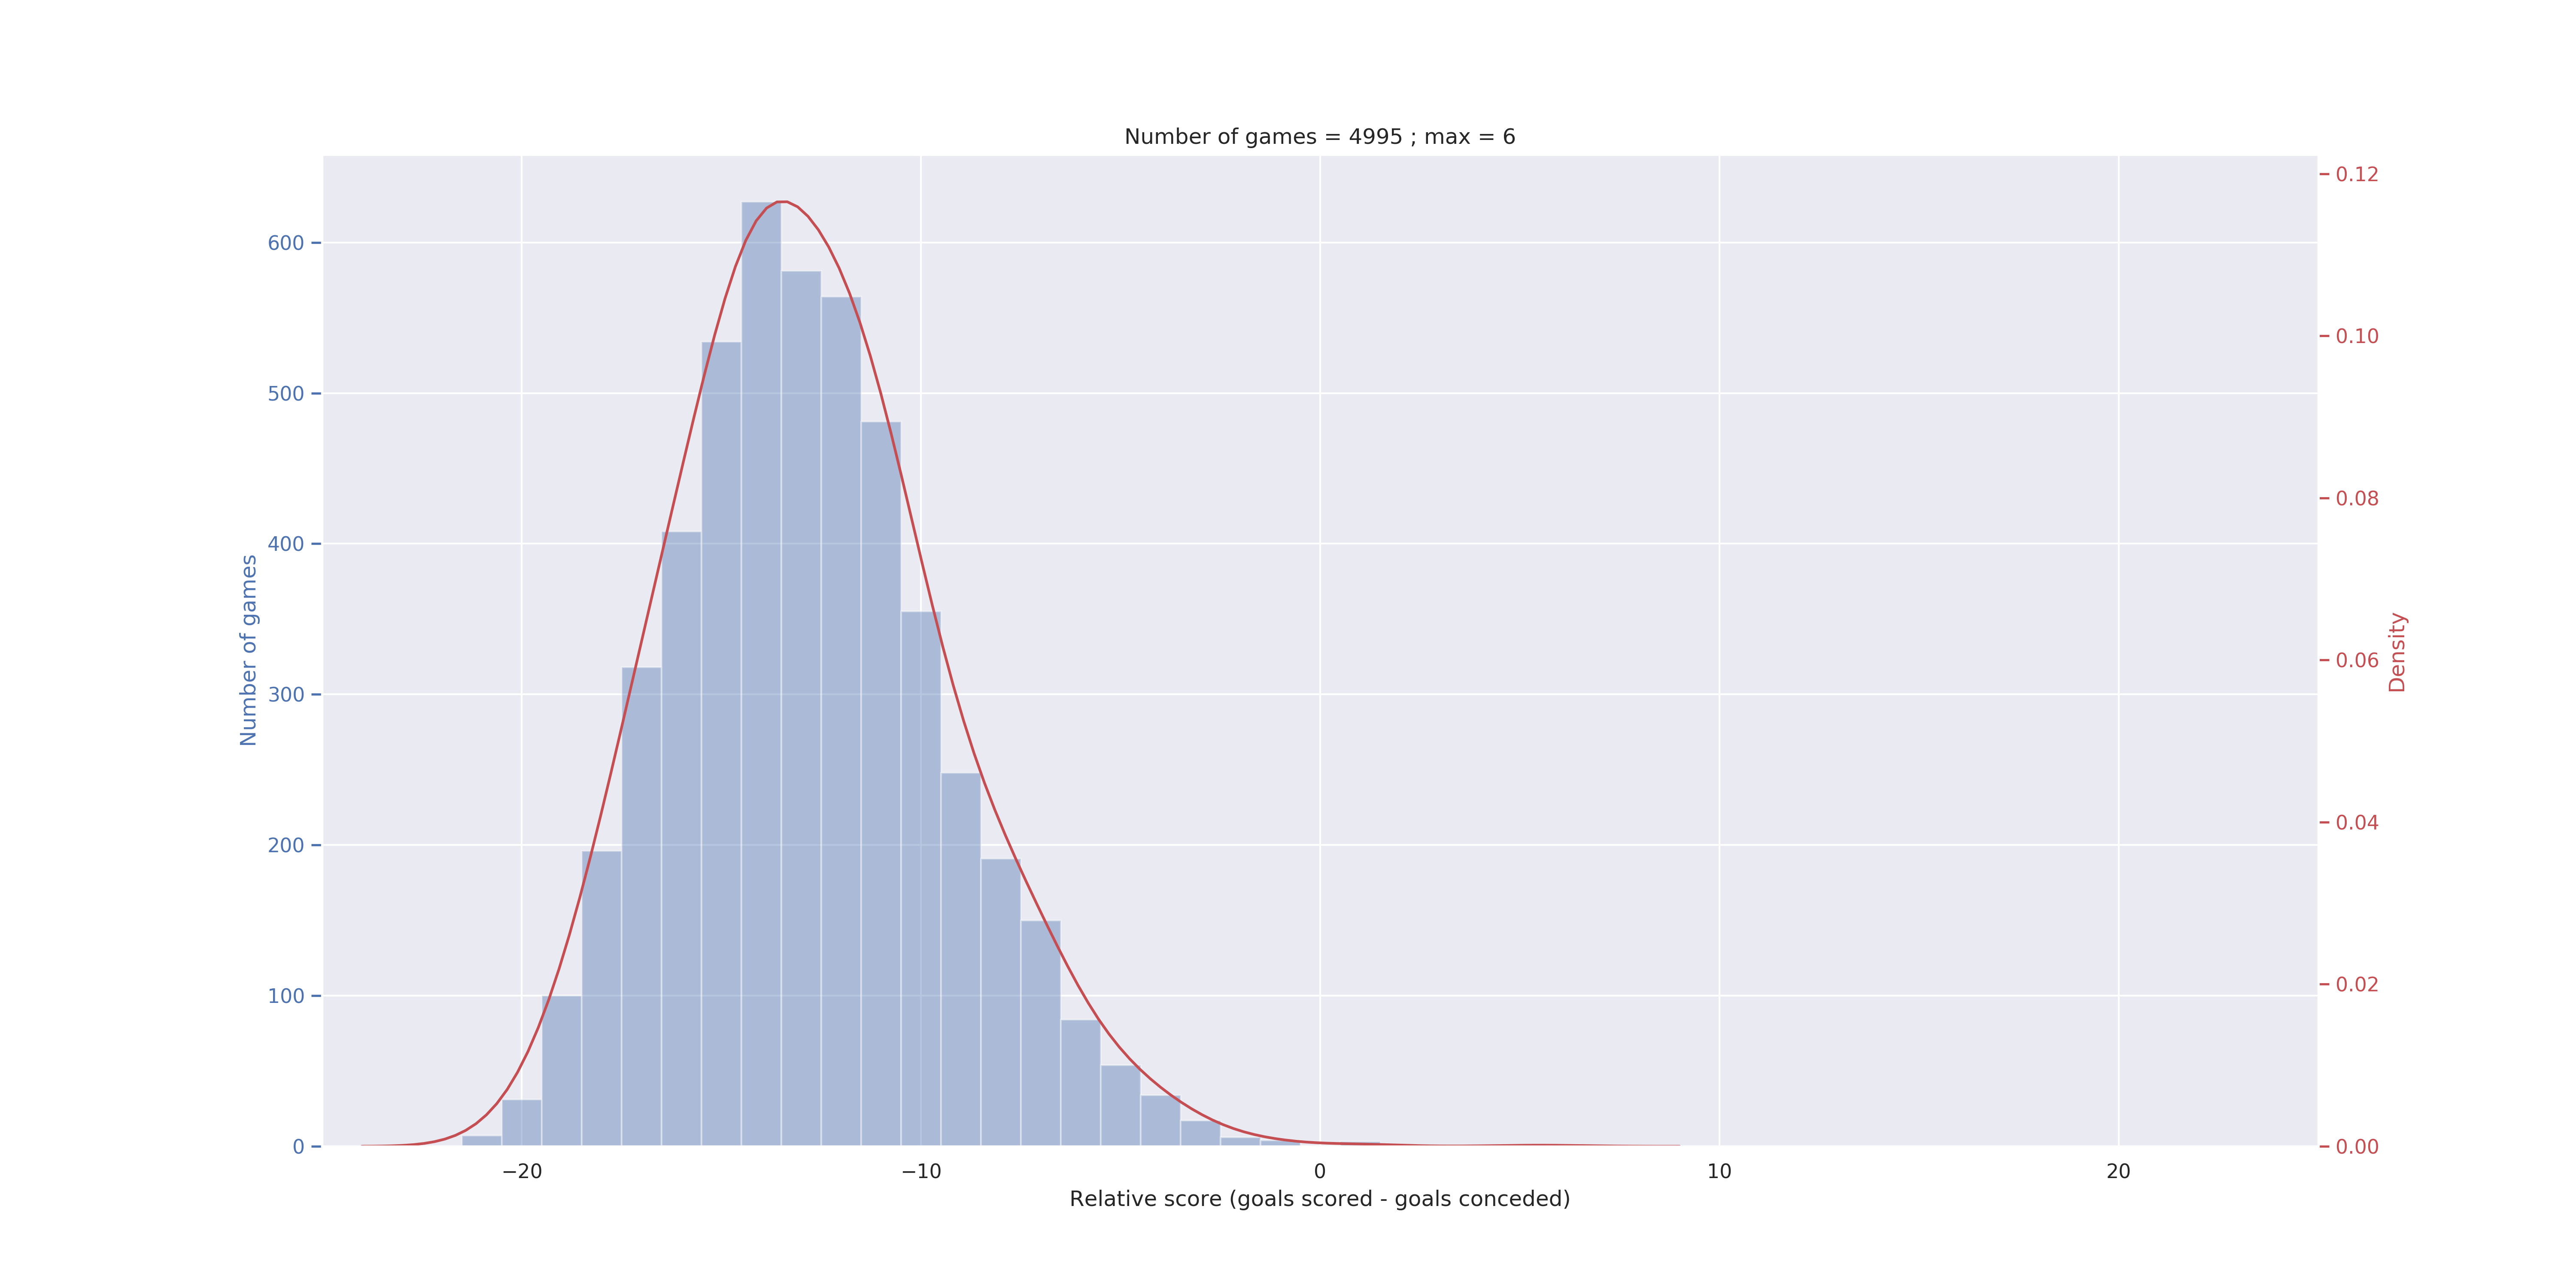
\includegraphics[width = \textwidth]{img/DQL_7000_withoutMax.png}
 \caption{Entraînement du Deep Q-Network sur 7000 parties sans Max pooling}
 \label{fig:DQL_7000_withoutMax}
\end{figure}

La figure \ref{fig:DQL_7000_withoutMax} nous présente l'histogramme obtenu. On constate qu'en moyenne notre réseau perd en marquant environ 7 ou 8 buts. Au-delà de 
10 buts marqués, la densité décroit fortement. On remarque cependant que cette décroissance n'empêche pas notre réseau d'avoir eu quelques très bons résultats.
Ainsi le repérage du maximum ($+\num{6}$) nous permet de conclure que notre réseau a réussi à gagner une partie avec le score 21--15. Nous avons donc là notre premier cas 
de victoires de notre IA ! Bien que celle-ci subit de nombreuses défaites (parfois cuisantes), ce résultat très encourageant confirme que nous sommes sur la bonne voie 
et que notre implémentation est correcte et relativement performante.

Le nombre important de défaites peut être expliqué par la grande dimension de notre espace. En effet, notre réseau est extrêmenent complexe et peut ajuster énormément 
de poids pour interpoler correctement notre fonction de satisfaction $Q$. Pour pouvoir entraîner correctement un tel réseau, il faudrait avoir un apprentissage assez 
long ou un taux d'apprentissage plus élevé. Nous n'augmentons pas le taux d'apprentissage pour ne pas altérer la stabilité de notre système. Une piste que nous
allons explorer par la suite est de rallonger l'apprentissage (à 15000 parties jouées). 

Avant cela, nous voulons étudier dans le même contexte (donc 7000 parties) un réseau plus modeste. Il s'agit du réseau avec les couches de max pooling. La dimension
de l'espace étant beaucoup plus faible, nous espérons une convergence plus rapide, et donc de meilleurs résultats après 7000 parties.

\begin{figure}[h]
 \centering
 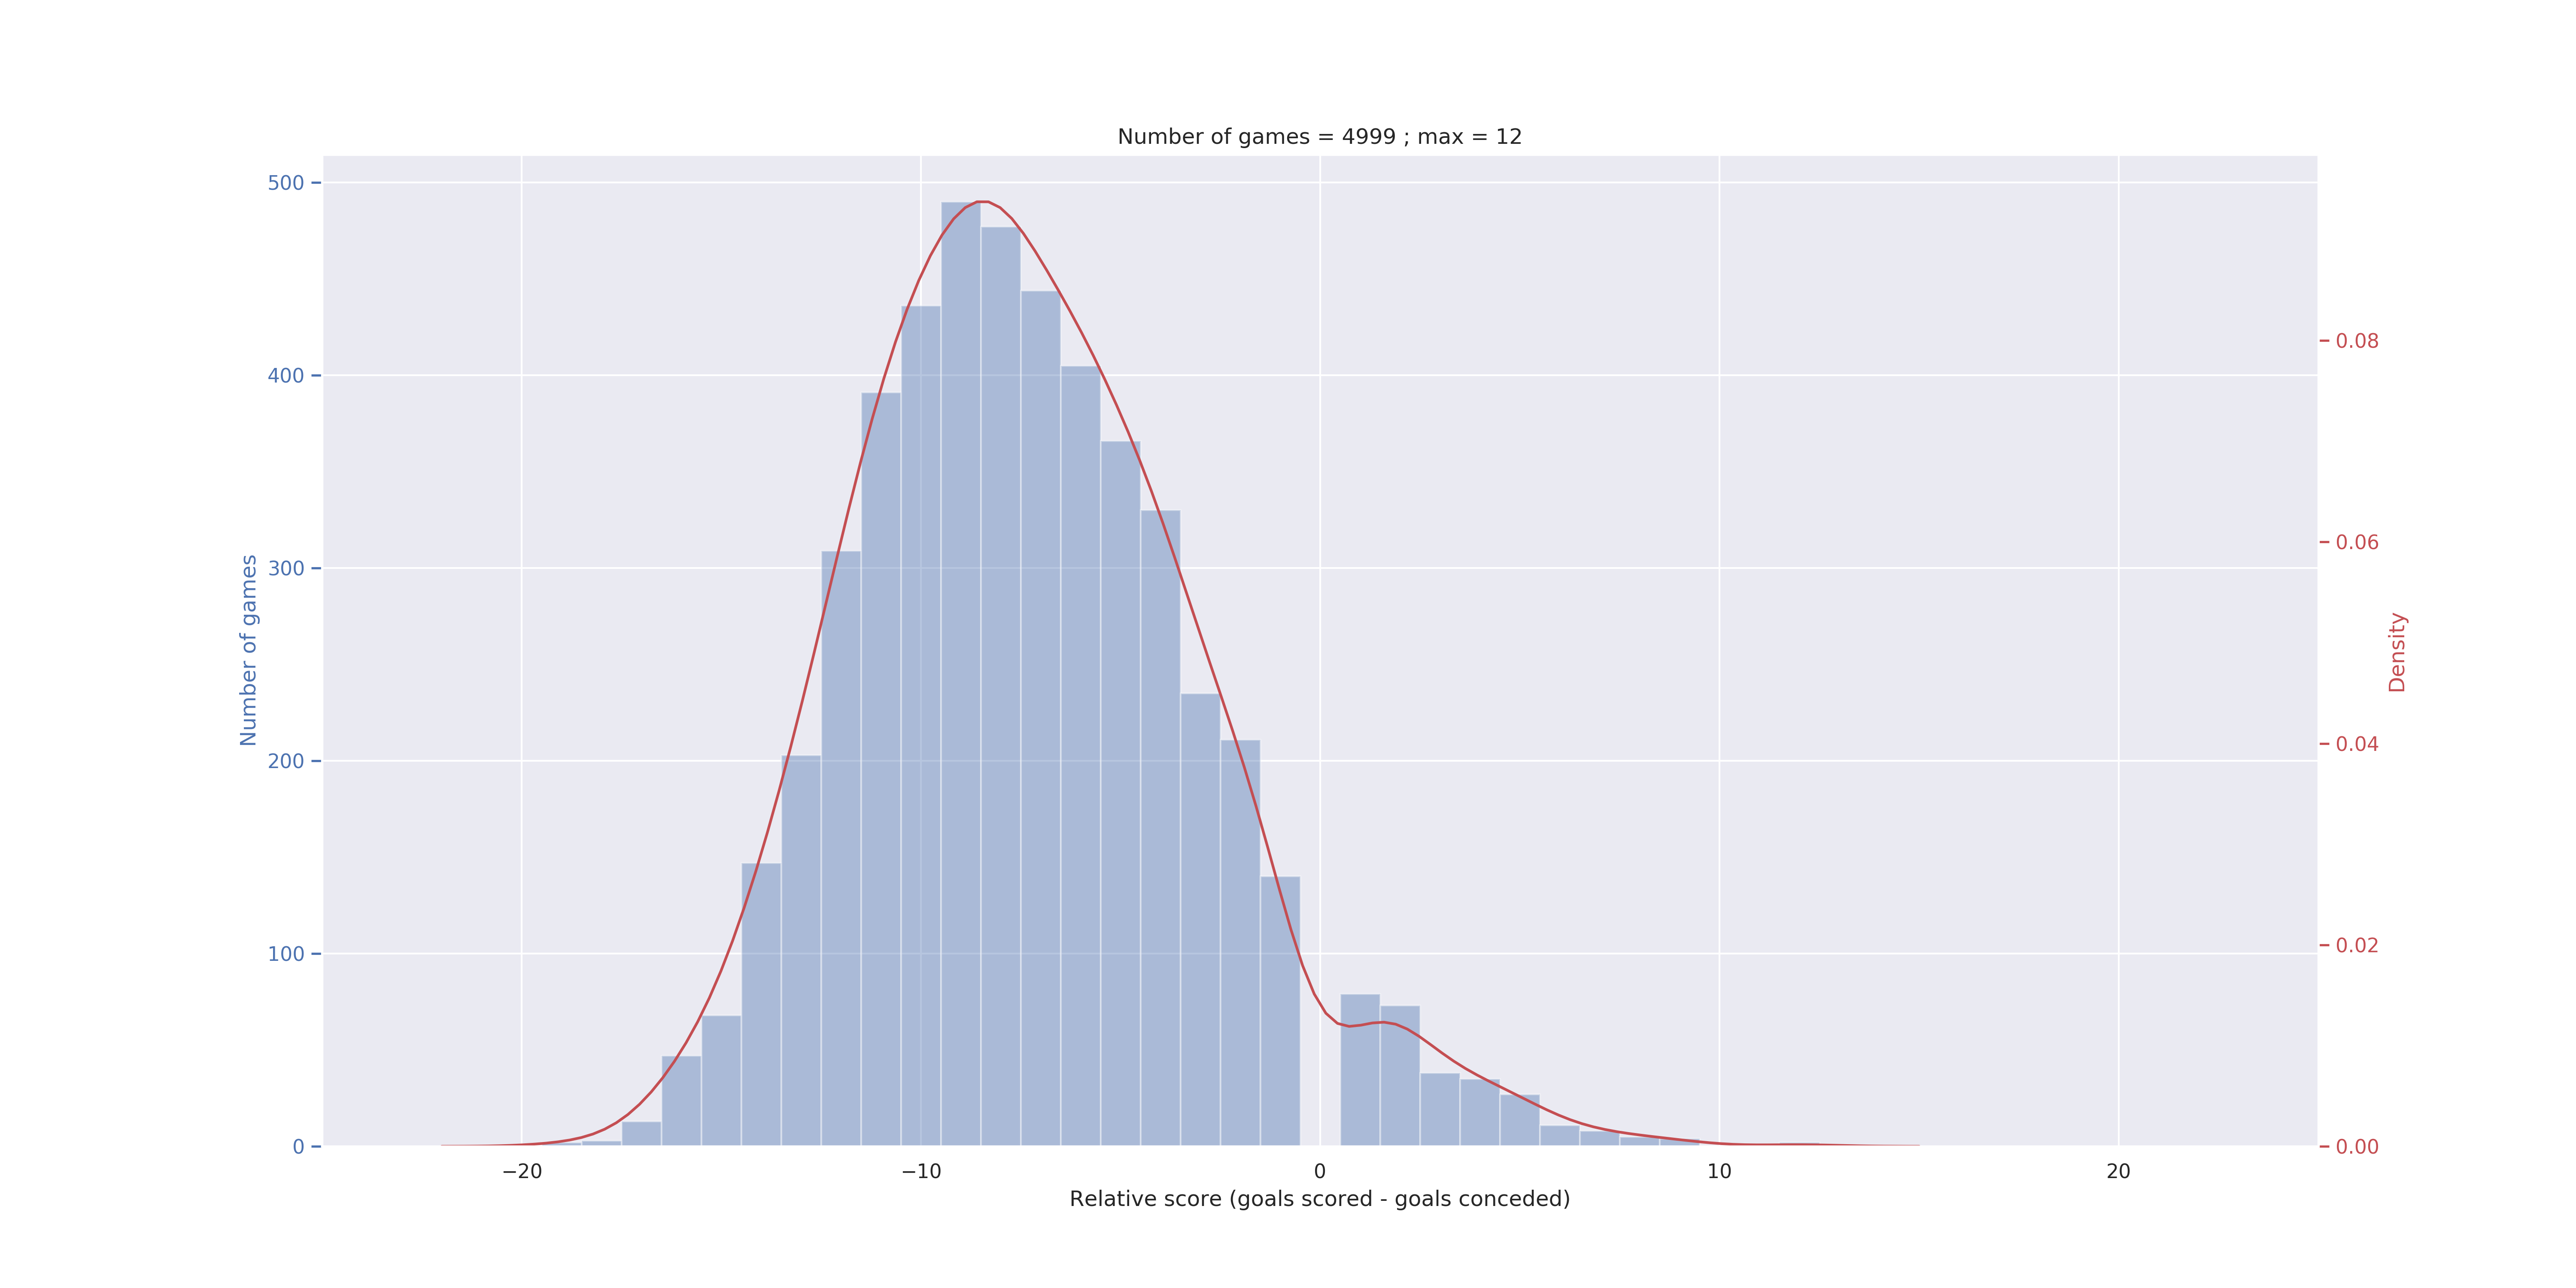
\includegraphics[width  = \textwidth]{img/DQL_7000_withMax.png}
 \caption{Entraînement du Deep Q-Network sur 7000 parties avec Max pooling}
 \label{fig:DQL_7000_withMax}
\end{figure}

Nos attentes sont confirmées par la figure \ref{fig:DQL_7000_withMax}. D'une part, le maximum est bien plus important : $+\num{12}$. Cela signifie que notre IA a 
réussi à remporter la victoire 21--9 face à son adversaire ! D'autre part, c'est la totalité de la distribution des scores qui est modifiée. En effet, on situe 
plus la moyenne vers $\num{-8}$ (soit une défaite 13--21). En outre, les scores relatifs positifs (correspondant donc à une victoire) sont bien plus fréquents. Ils
étaient totalement négligeables sur la figure \ref{fig:DQL_7000_withoutMax}. Ils sont désormais visibles bien que minoritaires. Cette IA se comporte
globalement mieux dans l'environnement Pong. Elle a mieux appris (probablement car la dimension de l'espace est bien plus faible) et est par suite bien plus forte
à ce jeu.

Notre objectif principal de ce projet est accompli ! Nous avons réussi à gagner à Pong grâce au Deep Q-Learning. Nos résultats demeurant toutefois imparfaits, nous
voulons étudier plus en profondeur l'apprentissage. Étant donné qu'un apprentissage sur Pong peut être très long, il nous est difficile de tester différentes
configurations pour mieux comprendre comme fonctionne le Deep Q-Learning. C'est pourquoi nous décidons de nous concentrer sur d'autres jeux que Pong.


\subsection{CartPole}

\subsubsection{Principe du jeu}

CartPole est un jeu disponible sur gym, représenté Figure \ref{fig:schema-cartpole}. Le principe est le suivant : on dispose d'un pendule simple fixé à sa base à un chariot. L'objectif est de stabiliser
le pendule en équilibre instable en déplaçant ledit chariot. Étant donné qu'apprendre un jeu à partir de photographies de l'écran est une contrainte très forte 
qui ralentit énormément l'apprentissage, nous préférons obtenir un espace des états plus petits pour pouvoir faire les tests voulus. CartPole nous donne un 
état à 4 dimensions (Figure \ref{fig:schema-cartpole-network}) composé de l'angle et la vitesse angulaire du pendule, et de la position et la vitesse du chariot.
Nous disposons de deux actions : aller à gauche ou à droite. Ne rien faire ne fait pas partie des actions disponibles.

CartPole est un jeu de survie. Pour survivre à une étape, le pendule ne doit pas être trop incliné, et le chariot ne doit pas être trop éloigné de sa position
initiale. Si notre IA survit 500 étapes, alors le jeu est réinitialisé. Cela permet de la remettre en difficulté dans le cas où l'IA a trouvé un
point stable. On considère que l'IA a réussi à jouer à CartPole si elle est capable de survivre 195 étapes. Cette limite est arbitraire mais souvent utilisée sur
Internet pour CartPole. Reprendre cette même convention nous permet de nous situer par rapport à autres réalisations que l'on peut trouver sur GitHub.

Pour résoudre ce jeu, il convient de trouver une fonction de satisfaction adéquate. Si l'on meurt, on reçoit bien évidemment une récompense négative, que nous
avons situé à $-1$. Nous voulons encourager notre IA à survivre, c'est pourquoi nous lui offrons une satisfaction pour le simple fait de rester en vie. Nous avons
décidé de donner une récompense de $1$ à chaque étape survécue.


\begin{figure}[h]
\centering
\begin{subfigure}{.3\textwidth}
  \centering
  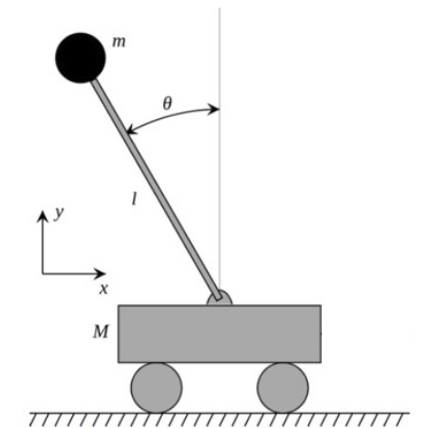
\includegraphics[width=.9\linewidth]{img/schema_cartpole.png}
  \caption{Schéma du jeu CartPole}
  \label{fig:schema-cartpole}
\end{subfigure}%
\begin{subfigure}{.6\textwidth}
  \centering
  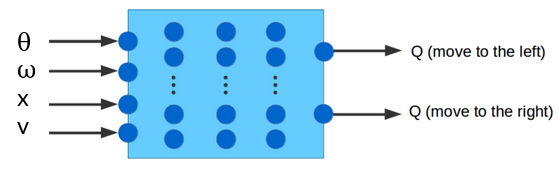
\includegraphics[width=.9\linewidth]{img/schema_cartpole_network.png}
  \caption{Espace des états sur CartPole}
  \label{fig:schema-cartpole-network}
\end{subfigure}
\caption{Représentation du jeu CartPole}
\label{fig:cartpole}
\end{figure}

\subsubsection{Apprentissage de CartPole}

Nous réalisons l'apprentissage sur CartPole. Le réseau utilisé est constitué de deux couches intermédiaires, toutes deux composées de 24 neurones. Les hyperparamètres
utilisés sont détaillés sur la figure \ref{fig:cartpole-2reseaux}.

\begin{figure}[h]
 \centering
 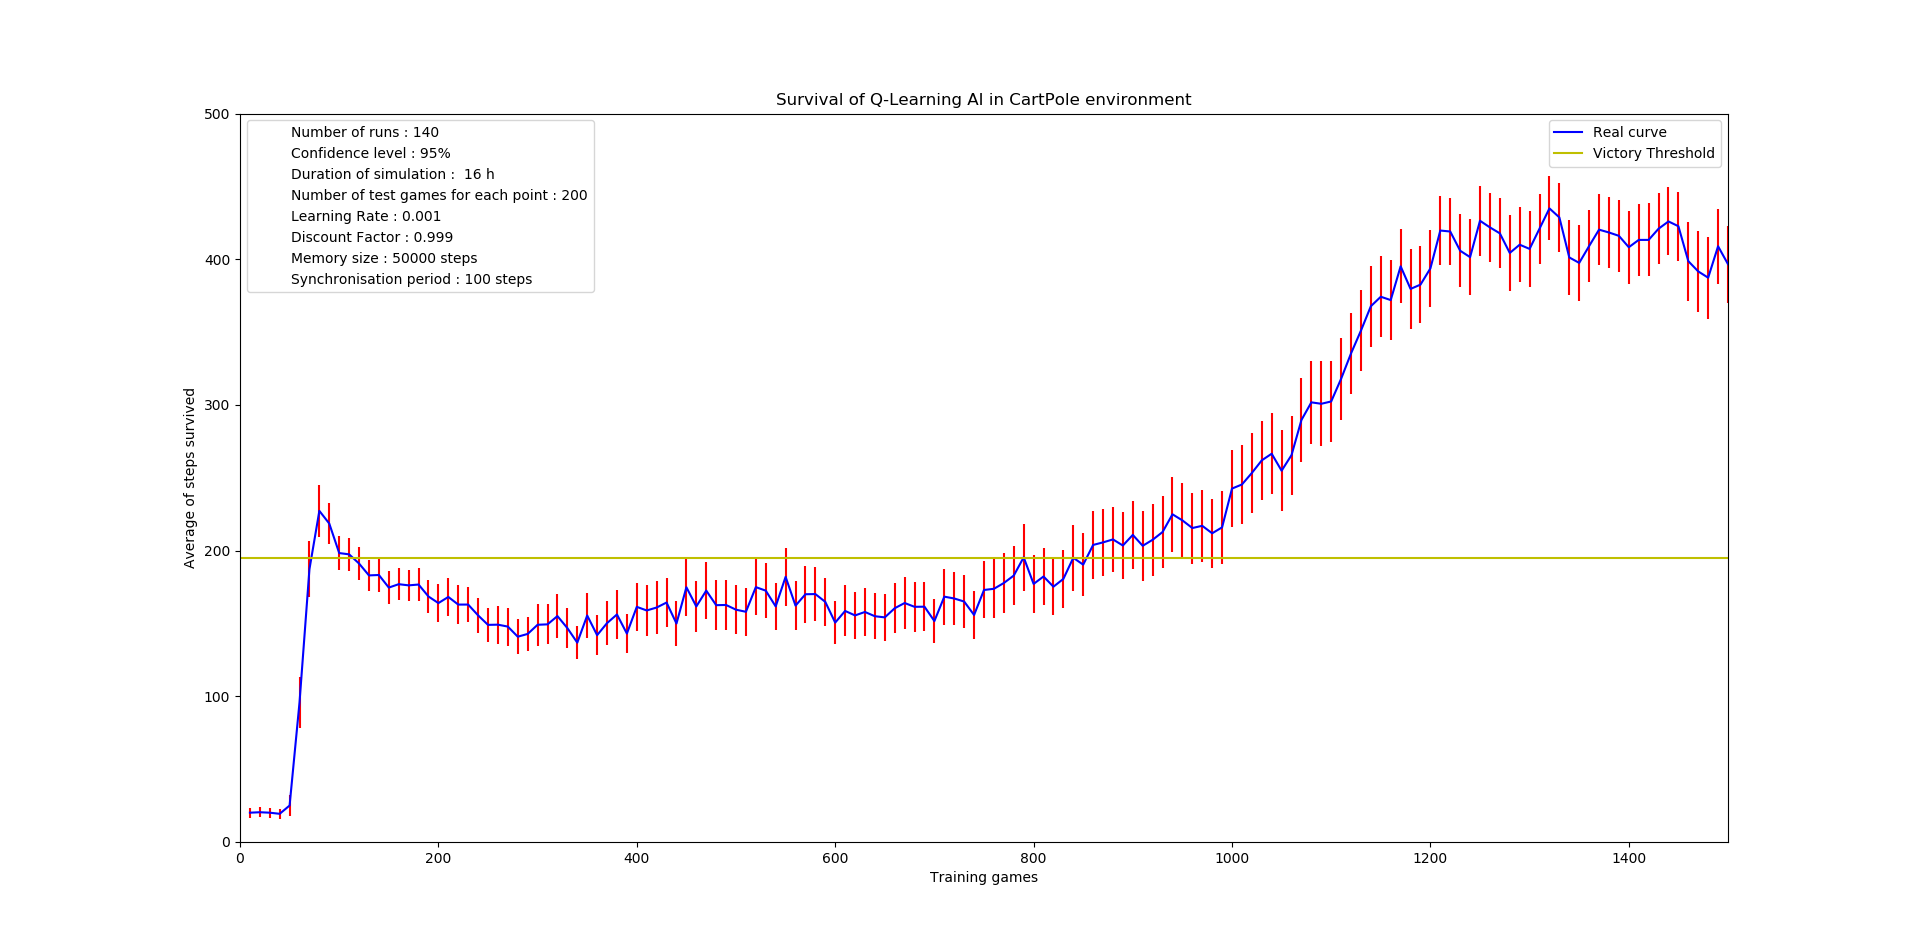
\includegraphics[width  = \textwidth]{img/cartpole_2reseaux.png}
 \caption{Apprentissage de CartPole}
 \label{fig:cartpole-2reseaux}
\end{figure}


On remarque que la barre des 195 étapes survécues a été franchi, ce qui signifie que l'on peut considérer que notre IA a réussi à apprendre CartPole.
Afin de pouvoir nous situer par rapport aux réalisations d'autres personnes sur GitHub, nous superposons notre courbe à celle obtenue avec un code disponible
sur GitHub.

\begin{figure}[h]
 \centering
 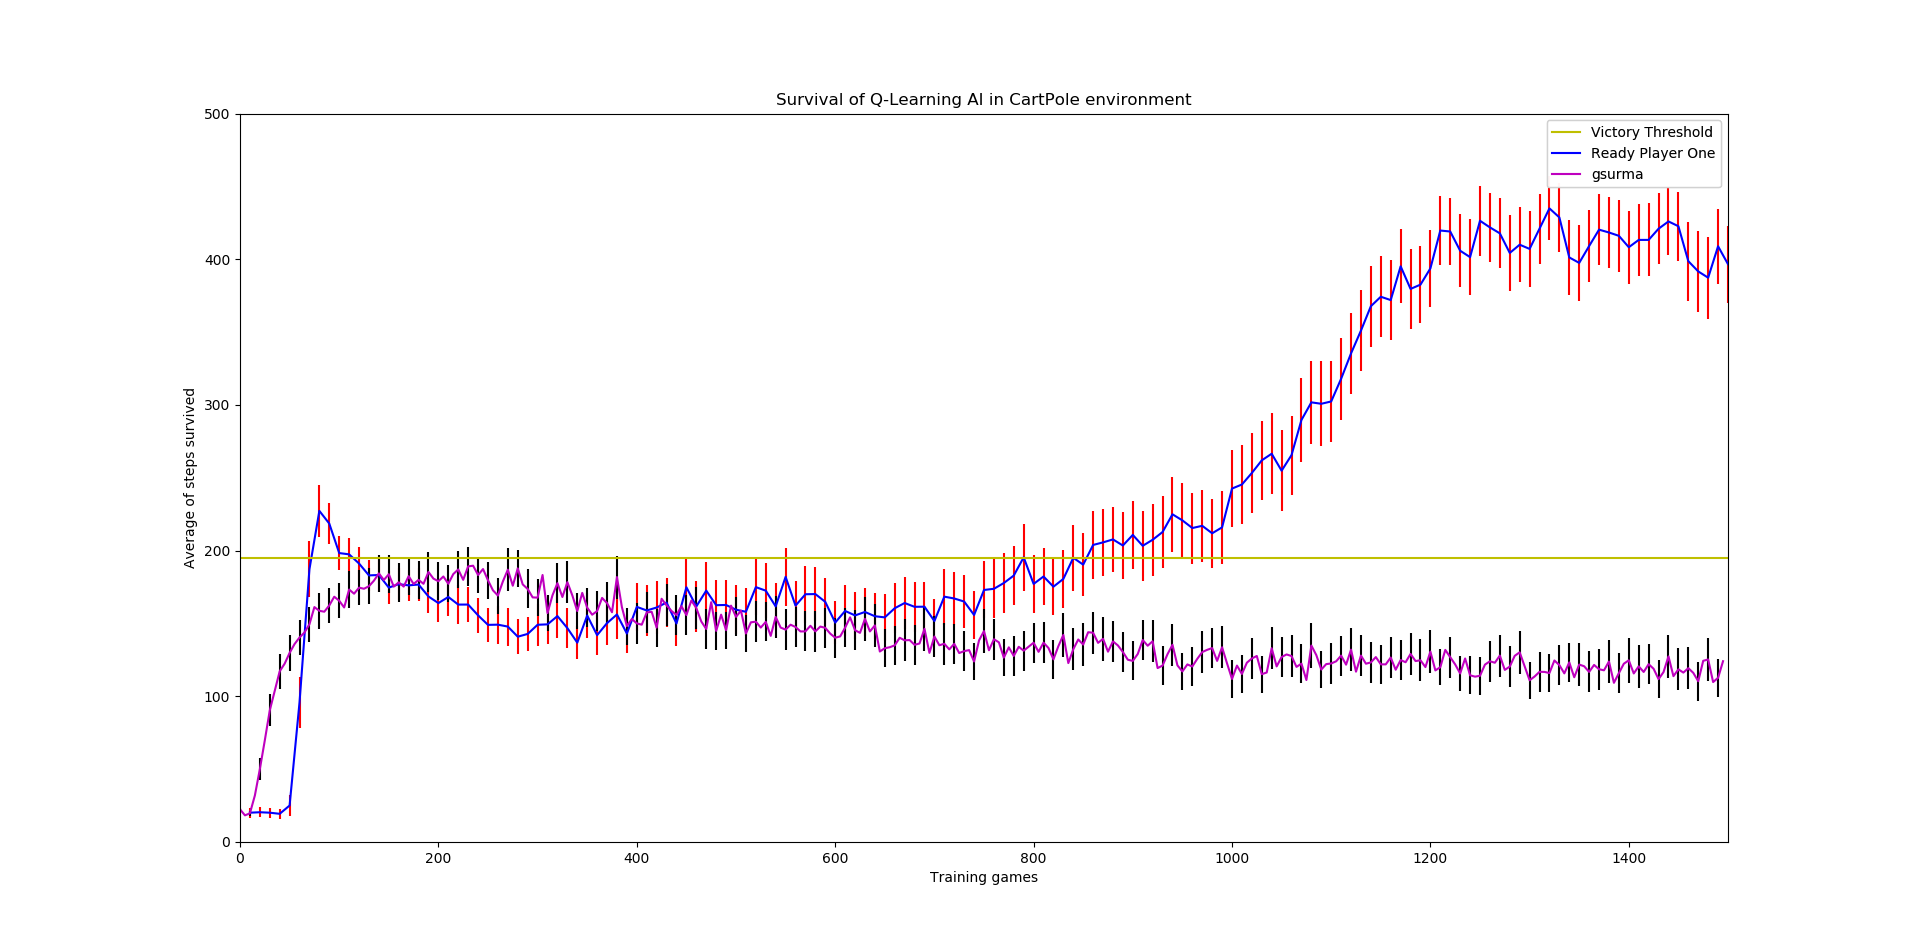
\includegraphics[width  = \textwidth]{img/gsurma.png}
 \caption{Comparaison des performances avec d'autres codes publics}
 \label{fig:gsurma}
\end{figure}

Le code public dépasse brièvement (et dans le meilleur des cas) la barre des 195 étapes survécues mais ne maintient pas ce résultat.
À l'instar de beaucoup d'articles scientifiques, seul le meilleur des cas permet de satisfaire les conditions de réussite, l'expérience étant arrêtée dès
que le jeu est résolu. En ce qui nous concerne, nous continuons l'expérience, ce qui nous permet de conclure sur la stabilité de notre algorithme. En outre,
nous moyennons nos résultats (en l'occurrence sur 140 réalisations) pour résoudre le jeu en moyenne et pas dans le meilleur des cas.

Sur GitHub, on a disposé deux vidéos après victoire de notre IA. La 
\href{https://raw.githubusercontent.com/ready-player-one-supelec/eponge-rapport/master/videos/balance.mp4}{première} 
montre un pendule qui survit mais demeure relativement chancelant. En poursuivant
l'apprentissage, on obtient la \href{https://raw.githubusercontent.com/ready-player-one-supelec/eponge-rapport/master/videos/equilibre.mp4}{seconde} vidéo. 
On remarque alors que notre IA trouve assez rapidement un point d'équilibre du pendule.

\subsubsection{Apprentissage avec un seul réseau}

Dans la section \ref{section:2networks}, nous avions expliqué que deux réseaux aidaient à stabiliser l'apprentissage, et qu'un seul réseau pouvait parfois mener à des
oscillations voire une instabilité de notre IA. Pour confirmer cela, nous avons voulu tester un apprentissage avec un seul réseau sur CartPole.
Le résultat est représenté figure \ref{fig:cartpole-1reseau}.

\begin{figure}[h]
 \centering
 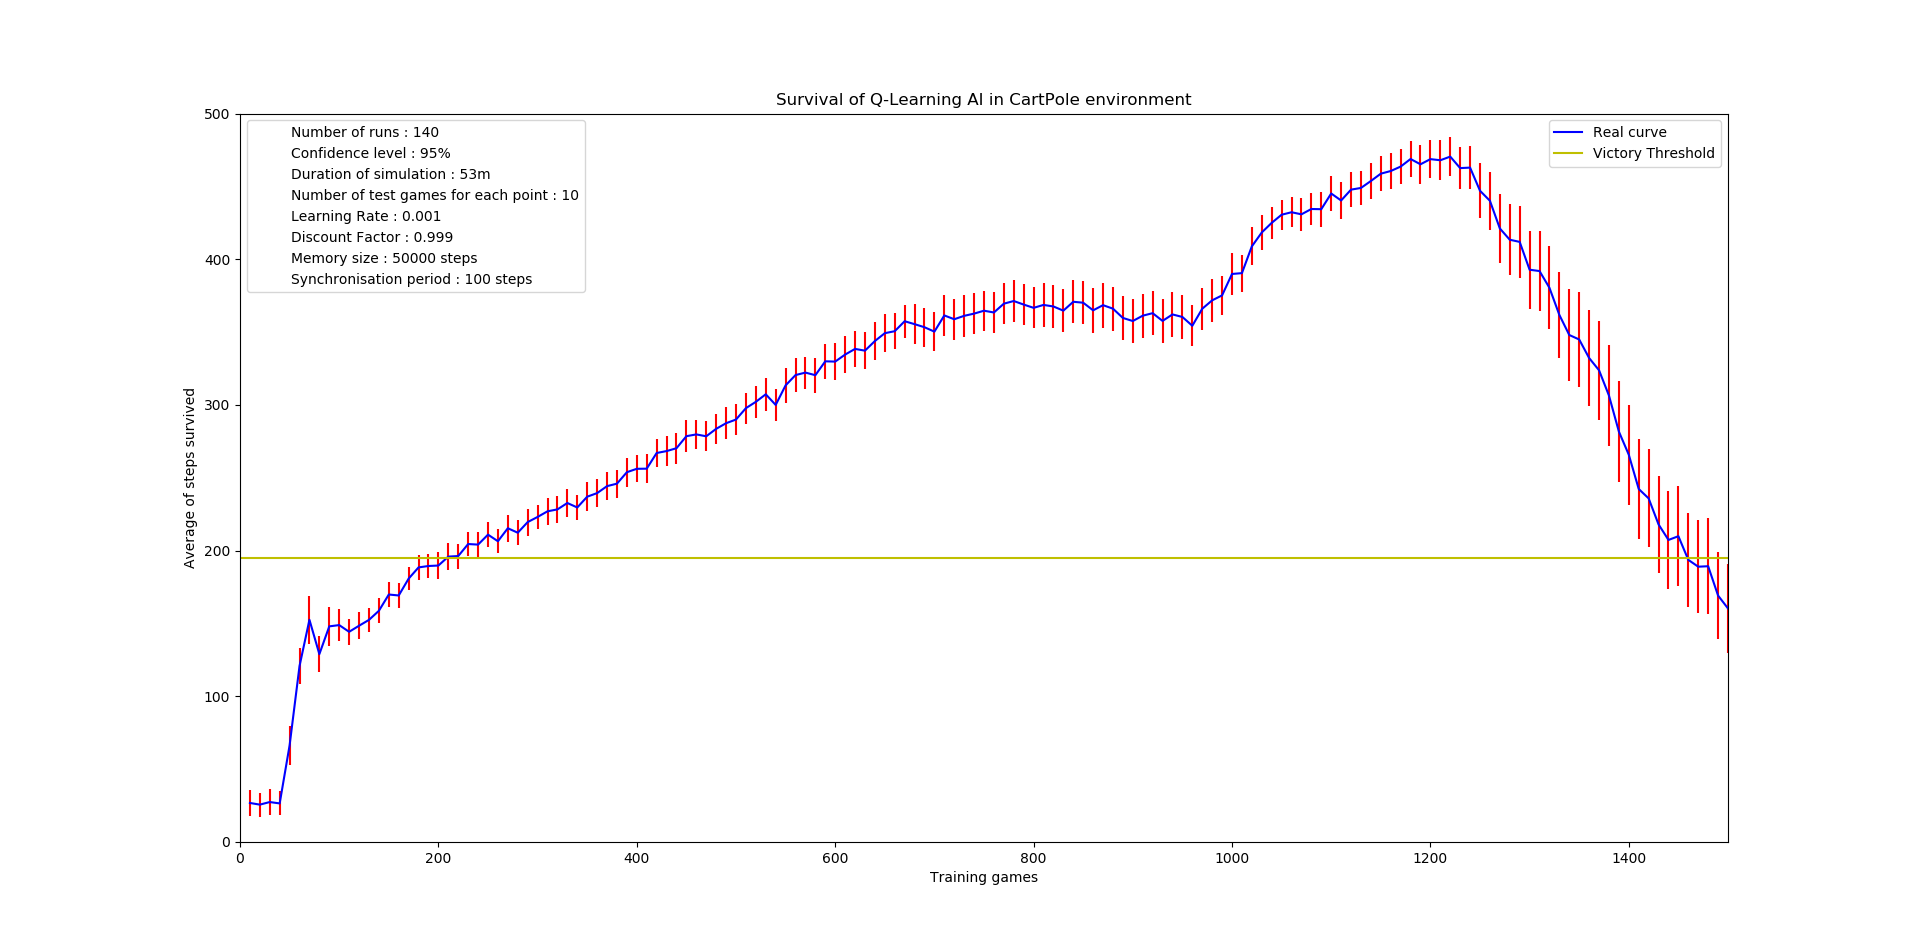
\includegraphics[width = \textwidth]{img/cartpole_1reseau.png}
 \caption{Apprentissage de CartPole avec un seul réseau}
 \label{fig:cartpole-1reseau}
\end{figure}

Nous remarquons une importante chute du temps de survie à la fin de l'apprentissage. Cela marque donc la forte instabilité de notre IA induite par le fait que le réseau
est unique. On remarque toutefois que le jeu est résolu et que l'on atteint des scores très élevées. Cela provient du fait que CartPole est un jeu suffisamment simple
pour qu'un seul réseau ne soit pas trop handicapant. Il est néanmoins suffisamment complexe pour faire apparaître l'intérêt d'un second réseau.


Puisqu'un apprentissage sur CartPole est relativement rapide, nous avons pu tester différentes configurations, et ainsi avoir une meilleure intuition des hyperparamètres
à choisir. Nous pouvons donc mettre cela en application avec un jeu un peu plus complexe : Flappy Bird.


\subsection{Flappy Bird}

\subsubsection{Principe}

Pour pouvoir manipuler la difficulté du jeu comme on le souhaite et pour avoir accès à l'espace des états que l'on veut, on a recréé le jeu Flappy Bird en C.
Notre IA dispose de deux actions possibles : bondir ou ne rien faire (et donc se laisser tomber).

Nous avons défini l'espace des états comme représenté figure \ref{fig:flappy-states}. Notre oiseau voit les données suivantes : la distance horizontale qui le sépare 
du prochain tuyau, les distances verticales qui le séparent du haut et du bas du passage, ainsi que du haut et du bas de l'écran, et sa vitesse verticale.
Toutes ces données ont été normalisées en prenant en compte les dimensions caractéristiques du jeu. 

\begin{figure}[h]
 \centering
 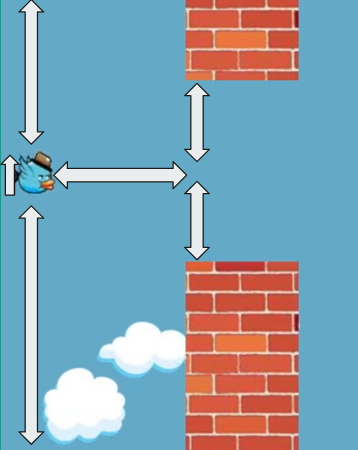
\includegraphics[scale = 0.3]{img/flappy_state.png}
 \caption{Illustration de l'espace des états de Flappy Bird}
 \label{fig:flappy-states}
\end{figure}

Nous devons également définir une fonction de récompense. Si l'oiseau meurt (sort de l'écran ou entre en collision avec un mur), la récompense est égale à $-1$.
Si l'on passe une porte, notre score est incrémenté et la récompense est égale à 1. Toutefois, pour que l'oiseau soit capable d'apprendre à passer les portes, il doit
tout d'abord réussir à en passer quelques unes par hasard afin qu'il comprenne que cette action rapporte des récompenses. Or, il est assez difficile d'avoir un 
score non-nul à Flappy Bird lorsqu'on joue aléatoirement. Pour encourager notre IA à vouloir rester en vie, on ajoute une composante survie à notre fonction de 
récompense. Ainsi, à chaque étape survécue, la récompense est de $0.1$.

\subsubsection{Apprentissage}

On réalise l'apprentissage du Flappy Bird que nous avons réalisé. Le réseau utilisé est constitué d'une couche intermédiaire de 16 neurones. Les hyperparamètres
utilisés sont les suivants : taux d'apprentissage à $0.001$, facteur d'actualisation à $0.99$, synchronisation des deux réseaux toutes les 500 étapes et décroissance
exponentielle du taux d'exploration.

On remarque que l'apprentissage est un succès. On obtient une IA capable de survivre à l'infini. On remarque également une certaine instabilité du réseau 
qui disparaît et ré-apparaît régulièrement à mesure que l'on poursuit l'apprentissage.

Ce résultat étant arrivé en fin de projet, nous n'avons pu tracer de courbes permettant de mieux cerner comme s'est déroulé l'apprentissage.
Toutefois, une vidéo de l'apprentissage est disponible sur \href{https://github.com/ready-player-one-supelec/eponge-rapport/blob/master/videos/flappy_cloud.mp4}{GitHub}.




